%!TEX root = ../thesis.tex
%*******************************************************************************
%****************************** Fourth Chapter *********************************
%*******************************************************************************

\chapter{Technological aspects} \label{c:4}

\ifpdf
	\graphicspath{{Chapter4/Figs/pdf/}}
\else
	\graphicspath{{Chapter4/Figs/svg/}}
\fi

\epigraph{`It is perfectly true, as the philosophers say, that life must be understood backwards. But they forget the other proposition, that it must be lived forwards.'}{Søren Kierkegaard, 1843 \cite{Kierkegaard1843}}

\subsection*{Declaration} 

\footnotesize

The content of this chapter was joint work with Tom Stubbs, with whom I designed and developed cuRRBS. Nevertheless, almost all the text, code and plots here presented were produced by myself. Additionally, I would like to recognise the contributions of Janet M. Thornton and Wolf Reik (who helped designing the study), Antonio J. M. Ribeiro (who implemented the last version of cuRRBS to make it more computationally efficient) and Felix Krueger (who processed the RRBS datasets). All of them also helped in the revision of the final text. This work has been published in the journal \textit{Nucleic Acids Research} \cite{Martin-Herranz2017a}.

\normalsize

\section{Background} \label{s:4.1}

\smallskip

With the advent of next-generation sequencing, scientists are studying the biology of life at unprecedented resolution \cite{Shendure2008}. Unfortunately, owing to the large size of many commonly studied genomes (human, mouse and tobacco plant for example are all > 2.5 \acrshort{Gbp} in size) \cite{Consortium2001,Consortium2002,Sierro2014}, it is often still prohibitively expensive to conduct whole genome sequencing at high coverage. This creates a trade-off that negatively impacts the number of replicates that can be included and, therefore, it challenges the statistical power and the reproducibility of the studies \cite{Fumagalli2013,Wu2015}. This is true in particular for \acrshort{DNA} methylation, where differentially methylated regions ( \acrshort{DMRs}) are typically called by identifying changes as small as $10\%$ and where $70-80\%$ of the reads of Whole Genome Bisulfite Sequencing (\acrshort{WGBS}) methods contain little to no relevant information on the DNA methylation status \cite{Ziller2013}.

\bigskip

To address these cost inefficiencies, many methods have been developed to \textbf{reduce the number of genomic fragments that need to be sequenced} for a given biological system \cite{Plongthongkum2014,Suzuki2013,Yong2016,Kurdyukov2016,Kacmarczyk2018}. These methods can be broadly split into those that positively select for genomic fragments of interest and those that deplete for fragments that are not of interest. Positive selection-based methods involve the sites of interest being enriched from the background. This usually occurs through pull-down of these sites via an antibody (e.g. anti-\acrshort{5mC} antibody) \cite{Taiwo2012}, a recombinant binding protein (e.g. methyl-\acrshort{CpG}-binding domains or \acrshort{MBD}) \cite{Brinkman2010}, covalent biotin tagging \cite{Kriukiene2013}, capture probes/baits for the sites of interest \cite{Ivanov2013,Allum2015,Cheung2017}, array-based approaches (e.g. \acrshort{27K}, \acrshort{450K} and \acrshort{EPIC} arrays in human) \cite{Bibikova2009,Bibikova2011,Pidsley2016,Hodges2009} or \acrshort{PCR}-based approaches \cite{Deng2009,Diep2012,Komori2011,Paul2014,Bernstein2015,Yang2015}. These methods have many limitations, including enrichment biases, complex protocols and difficulties in quantification \cite{Suzuki2013,Yong2016}.

\bigskip 

Current evidence shows that depletion-based methods do not have enrichment biases, tend to be simpler and are more readily quantifiable \cite{Suzuki2013,Kurdyukov2016}. The most common depletion-based approaches use restriction enzymes to exploit the fact that the nucleotide composition in a given genome is non-random and that the fragment lengths produced from a given digestion will thus reflect this \cite{Cedar1979,Cohen-Karni2011,Bystrykh2013,Martinez-Arguelles2014,Yu2004}. In the case of 5-methylcytosine (5mC), the most common depletion-based method is Reduced Representation Bisulfite Sequencing (\acrshort{RRBS}) using the methylation-insensitive restriction enzyme MspI (with the recognition sequence C|CGG) \cite{Meissner2008,Boyle2012}, although enzymes such as BglII \cite{Meissner2005}, XmaI \cite{Tanas2017}, Taq$^\alpha$I \cite{Lee2014,Lim2016}, MspJI \cite{Huang2013} , ApeKI \cite{Wang2013}, HpyCH4IV or HpaII \cite{Kirschner2016} have also been used. RRBS has proven extremely useful for cost-effective, global studies of DNA methylation \cite{Stubbs2017,Meissner2008,Lee2014,Gu2010}, capturing around $10\%$ of CpG sites within mammalian genomes but with up to a 30-fold reduction in the number of fragments sequenced in comparison to WGBS \cite{Smith2009}. 

\bigskip

In the context of epigenetic clocks, most studies have used methylation arrays in humans \cite{Horvath2013,Hannum2013,Koch2011} and MspI-based RRBS in mice, dogs and wolves \cite{Stubbs2017,Petkovich2017,Thompson2018,Meer2018,Thompson2017}. The utility of the MspI-based RRBS approach is limited to a specific subset of CpG sites in the genome, mainly found within CpG islands and promoters \cite{Meissner2008}. Nevertheless, it is known that many age-related changes in the methylome occur in other genomic regions (such as enhancers) \cite{Slieker2016,Slieker2018,Cole2017,Martin-Herranz2019a}, and current technologies could be biasing our discoveries. Furthermore, epigenetic clocks could be used in the near future to perform high-throughput screenings of anti-ageing drugs or employed as ageing biomarkers in clinical trials \cite{Horvath2018a}. However, the current assay costs could preclude the use of epigenetic clocks in this context.

\bigskip 

Given that restriction enzyme-based approaches are versatile and simple, we developed a new computational method called \textbf{customised Reduced Representation Bisulfite Sequencing} (\acrshort{cuRRBS}), which allows researchers to optimise the RRBS protocol for a specific experiment. cuRRBS generalises the problem of genomic enrichment with restriction enzymes by allowing the user to define both the genome and the particular sites of interest, before outputting the optimal enzyme combinations and size ranges to target these sites. In addition, cuRRBS provides the user with a variety of metrics to compare the various suggested protocols, including an estimate of the fold-reduction in sequencing costs compared to WGBS and a robustness value to assess the impact of experimental error in the size selection step.

\bigskip

Here, we have tested the enrichment ability of cuRRBS in several biological systems (including the Horvath epigenetic clock), with sites in both CpG and \acrshort{CHG} contexts and multiple species, to showcase the generalisability and utility of the software \cite{Horvath2013,Hanna2016,Milagre2017,Kawakatsu2016,Maurano2015,LevMaor2015,Domcke2015}. In addition, we take advantage of two recently published independent RRBS datasets to demonstrate the accuracy of the software predictions in both single and double enzyme experimental settings \cite{Tanas2017,Lim2016}. We hope that cuRRBS will be useful as a tool for designing cost-effective, genome-wide studies in the future, to help in the development of new epigenetic-based predictors and to validate previous results from whole genome approaches in a simple, cheap and timely fashion.

\smallskip

\section{Restriction enzyme digestion as a tool for genomic enrichment}

\smallskip

Restriction enzymes represent an incredibly effective tool for the enrichment of certain sites of interest in a genome. This is possible due to the wide variety of motifs that commercially-available restriction enzymes can recognise (Fig.~\ref{fig:c4_fig1}) combined with the non-random nature of the genome composition itself. Fig.~\ref{fig:c4_fig1} highlights that this motif diversity is driven both by the sequence composition (\acrshort{GC content}) and the length of the recognition sequence. Thus, different restriction enzymes will generate different fragment length distributions, dependent upon how frequently their recognition site is present in a given genome (Fig.~\ref{fig:c4_fig2}a, Fig.~\ref{fig:sc4_fig1}).

\vspace{3.5mm}


\begin{figure}[htbp!] 
	\centering    
	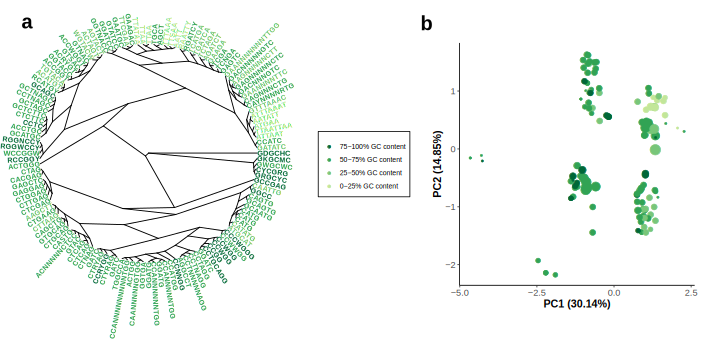
\includegraphics[width=1.0\textwidth]{C4_Fig1}
	\caption[The landscape of restriction enzyme motifs]{The landscape of restriction enzyme motifs. \textbf{a.} Phylogenetic analysis of the motifs that are recognised by the different commercially-available restriction enzymes which are insensitive to CpG methylation. Each sequence represents a different isoschizomer family considered in this study. A neighbour-joining method was used to construct the tree. Motifs with different GC content are shown with different colours. \textbf{b.} Principal component analysis (\acrshort{PCA}) performed on the matrix of pairwise distances from the aligned motifs. Each circle represents a different motif. The coordinates of the different motifs on the first two principal components are plotted on the x- and y-axes. Motifs with different GC content are shown with different colours (same as in a.) and the motif length is represented by the diameter of the circle.}
	\label{fig:c4_fig1}
\end{figure}


\begin{figure}[htbp!] 
	\centering    
	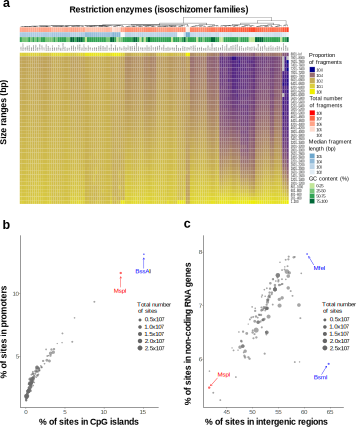
\includegraphics[scale=1.4]{C4_Fig2}
	\vspace*{3mm}
	\caption[Restriction enzyme digestion as a tool for genomic enrichment]{Restriction enzyme digestion as a tool for genomic enrichment. \textbf{a.} Heatmap showing the fragment length distributions generated by different restriction enzymes in the human genome (\acrshort{hg38}). Each column represents the distribution for an isoschizomer family of restriction enzymes that contains at least one member which is methylation-insensitive in a CpG context. The distributions are binned in size ranges of 200 \acrshort{bp}, ordered as they would appear in an electrophoretic gel. Additional row annotations on top of the heatmap contain information regarding the total number of fragments (in red) and the median fragment length (in blue) produced by each in silico digestion, together with the GC content of the recognition motif in the isoschizomer family (in green). Legend is displayed on the right hand side. \textbf{b.} Scatterplot showing the percentage of cleavage sites from different restriction enzymes that overlaps with CpG islands (x-axis) and promoters (y-axis) in the human genome (hg38). The size of the circles represents the total number of cleavage sites generated by each enzyme. The enzymes MspI and BssAI are highlighted in red and blue respectively. Legend is displayed on the right hand side. \textbf{c.} Scatterplot showing the percentage of cleavage sites from different restriction enzymes that overlaps with intergenic regions (x-axis) and non-coding \acrshort{RNA} genes (y-axis) in the human genome (hg38). The size of the circles represents the total number of cleavage sites generated by each enzyme. The enzyme MspI is highlighted in red. The enzymes BsmI and MfeI are both highlighted in blue. Legend is displayed on the right hand side.}
	\label{fig:c4_fig2}
\end{figure}


In DNA methylation studies the most common application is the use of MspI (cutting at C|CGG) in RRBS (Reduced Representation Bisulfite Sequencing), which is used to enrich for CG dinucleotides (CpGs) contained in promoters and CpG islands \cite{Meissner2008} (Fig.~\ref{fig:c4_fig2}b). However, in many cases, MspI is by no means the most effective restriction enzyme that could be used. For instance, MspI would be a poor restriction enzyme to choose for the enrichment of CpGs found in intergenic regions or non-coding RNA genes, which would be far better enriched for using BsmI or MfeI respectively (Fig.~\ref{fig:c4_fig2}c). In fact, it turns out that across many genomic features MspI is rarely the most optimal methylation-insensitive restriction enzyme (Fig.~\ref{fig:sc4_fig2}). 

\bigskip

Previous studies have tested the potential of other restriction enzymes and enzyme combinations to expand the range of CpG sites that can be targeted in a genome \cite{Cedar1979,Bystrykh2013,Martinez-Arguelles2014,Yu2004,Tanas2017,Lee2014,Wang2013,Kirschner2016}. However, to our knowledge, there is currently no computational method that systematically explores the capacity of all commercially-available restriction enzymes to generate `personalised' reduced-representations of the genome whilst minimising the experimental cost (Fig.~\ref{fig:sc4_fig3}).

\smallskip

\section{cuRRBS: customised Reduced Representation Bisulfite Sequencing}

\smallskip

We have developed a novel computational method (cuRRBS) that determines the optimal combination of restriction enzymes and size range to enrich for any given set of sites of interest in any genome. In other words, by modifying two of the steps in the original RRBS protocol (Fig.~\ref{fig:c4_fig3}a), cuRRBS generalises RRBS.

\bigskip

The software takes as input the genomic coordinates that the user wants to target (Fig.~\ref{fig:c4_fig3}b, Fig.~\ref{fig:sc4_fig4}a). Afterwards, cuRRBS assesses \textit{in silico} the potential of all single enzymes and double-enzyme combinations to enrich for the sites of interest using the following variables:

\begin{itemize}
	
	\item \textit{\acrshort{NF}}, which reflects the theoretical number of genomic fragments that will be sequenced after the size selection step (i.e. those whose lengths after the \textit{in silico} digestion are within the size range). Assuming that the sequencing cost is proportional to \textit{NF}, cuRRBS attempts to minimise this value.
	
	\item \textit{Score}, which reflects the theoretical number of sites of interest that will be sequenced after the size selection step. cuRRBS attempts to maximise this value, which can be calculated as:
	
	\begin{align}
	Score = \sum_{i=1}^{n} w_i \cdot \gamma_i
	\end{align}
	
	where $n$ is the total number of sites of interest, $w_i$ is the weight of the $i$th site of interest and $\gamma_i$ is 1 if the $i$th site would be theoretically sequenced (i.e. present in a size selected fragment and $\leq$ \textit{read length} base pairs away from one of the ends of the fragment) and 0 otherwise.
	
	\item \textit{Enrichment Value} (\textit{\acrshort{EV}}), which combines both \textit{NF} and \textit{Score} into a single number. The objective of cuRRBS is to minimise \textit{EV}, which can be calculated as:
	
	\begin{align}
	EV = -log_{10} \left(\frac{Score}{NF} \cdot \frac{n}{max\_Score}\right)
	\end{align}

	where $max\_Score$ is the \textit{Score} obtained if all the sites of interest were sequenced.
	
\end{itemize}


The $NF$ and $Score$ variables are positively correlated with one another, such that the more genomic fragments sequenced, the more sites of interest are likely to be contained within the reduced representation (Fig.~\ref{fig:c4_fig3}c, Fig.~\ref{fig:sc4_fig4}b). However, this relationship disappears at higher $NF$ values, where the $Score$ variable becomes saturated such that any additional fragments sequenced will result in a reduction in the overall enrichment of the sites of interest. This $Score$ saturation at high $NF$ is mainly due to additional sites of interest being buried within long fragments that will not be sequenced due to limitations in the read length (cuRRBS parameter –r, see Table~\ref{table:c4_table1}). For a given enzyme or enzyme combination, the $NF$ and the $Score$ variables depend on the \textit{size range} chosen, since only the genomic fragments within the size range will be present in the reduced representation of the genome. 

\bigskip

cuRRBS requires that the user sets \textit{thresholds} for the maximum $NF$ (i.e. minimum \textit{\acrshort{CRF}}, see below) and minimum $Score$ that would be acceptable for a given application (Fig.~\ref{fig:c4_fig3}b, Fig.~\ref{fig:sc4_fig4}a). These \textit{thresholds} allow cuRRBS to search through all possible \textit{size ranges} for a given enzyme or enzyme combination and to find the one that minimises the \textit{Enrichment Value} ($EV$). cuRRBS repeats this procedure for every single enzyme and enzyme combination and reports those with the best hits (i.e. those with the lowest $EV$s) (Fig.~\ref{fig:sc4_fig4}a).

\bigskip

The output file contains the best scoring enzymes with their correspondent size ranges and some other useful variables for each one of the hits, such as:

\begin{itemize}

	\item \textit{Cost Reduction Factor} (\textit{CRF}), which estimates the theoretical fold-reduction in sequencing costs for the cuRRBS protocol when compared to Whole Genome Bisulfite Sequencing (WGBS). The \textit{CRF} for a given cuRRBS protocol can be calculated as:
	
	\begin{align}
	CRF = \frac{NF_{ref}}{NF} =  \frac{g/r}{NF}
	\end{align}
	
	where $NF_{ref}$ is the estimated number of fragments that would be sequenced in a WGBS experiment, that can be roughly calculated as the genome size ($g$) divided by the read length ($r$).
	
	\item \textit{Robustness} (\textit{\acrshort{R}}). This assesses how much the cuRRBS prediction varies if a slightly different size range is used (Fig.~\ref{fig:c4_fig3}d). The results for robust enzymes will not be greatly affected as a consequence of experimental error during the size selection step. This will help the user to make an informed decision on which enzyme combination to choose for the system of interest (Fig.~\ref{fig:sc4_fig4}c).	The \textit{robustness} of a given enzyme (combination) is calculated as:
	
	 \begin{align}
	 R = e^{-\theta}	
	 \end{align}
	 
	 with
	 
	 \begin{align}
	 \theta = \frac{\sum_{x\in\{a-\delta,a,a+\delta\}} \sum_{y\in\{b-\delta,b,b+\delta\}} |EV_{x,y} - EV_{a,b}|}{EV_{a,b}}
	 \end{align}
	 
	 where $EV_{a,b}$ is the $EV$ for the optimal size range ($a$: lower limit in size range, $b$: breadth) and $\delta$ is the experimental error (in bp) that is assumed during the size selection step. The \textit{robustness} will take values in the interval $(0,1]$, with higher values identifying robust cuRRBS protocols.
	
\end{itemize}



\begin{figure}[htbp!] 
	\centering    
	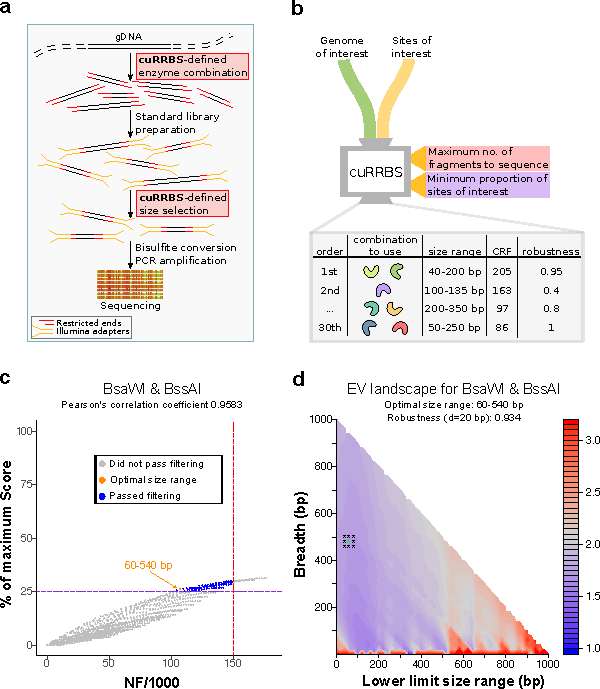
\includegraphics[width=0.9\textwidth]{C4_Fig3}
	%\vspace*{3mm}
	\caption[cuRRBS overview]{cuRRBS overview. \textbf{a.} Outline of an RRBS protocol. Highlighted are the two steps that would be modified according to the output produced by cuRRBS (i.e. the restriction enzymes used for the genomic digestion and the size selection). Legend is displayed on the bottom left. \textbf{b.} Schematic of cuRRBS. Highlighted are the two main inputs required for the software and the two \textit{thresholds} that the user has to define (red and purple tags). The default output for cuRRBS is a table containing the top hits (restriction enzyme combination and size range) along with additional information that might be useful to the user (such as \textit{Cost Reduction Factor} and \textit{robustness}). \textbf{c.} Scatterplot showing the trade-off between the number of fragments (\textit{NF}) and the \textit{Score} for the best enzyme combination (BsaWI \& BssAI) that targets the CpGs present in the human placental-specific imprinted regions \cite{Hanna2016}. \textit{NF} is divided by 1000 for visualization purposes. Each point represents a different \textit{size range}. Shown in dark blue and grey are the size ranges that would and would not pass filtering respectively. Shown in orange is the optimal size range in the filtered search space. The dotted lines depict the \textit{thresholds} that need to be specified by the user (red: maximum \textit{NF}; purple: minimum percentage of the maximum \textit{Score}). In this mock example we specified an \textit{NF threshold} of 150000 fragments and a \textit{Score threshold} of $25\%$ of the maximum \textit{Score}. Legend is displayed below the plot title. \textbf{d.} Contour plot that depicts how the \textit{robustness} (\textit{R}) variable is calculated for the optimal enzyme combination (BsaWI \& BssAI; size range: 60-540 bp) that targets the CpGs present in the human placental-specific imprinted regions \cite{Hanna2016}. \textit{Enrichment values} (\textit{EVs}) are calculated for all possible size ranges in order to create an \textit{EV} `landscape'. In this landscape, cuRRBS finds the size range with the lowest \textit{EV} that still satisfies the \textit{thresholds} (asterisk in green). Afterwards, cuRRBS samples \textit{EV}s around the optimum (asterisks in black). The points that are sampled depend on the experimental error (in this case, $\delta = 20$ bp). A high \textit{robustness} value means that the sampled \textit{EV}s do not change a lot when compared to the optimum, which implies that cuRRBS prediction will not be greatly affected by experimental errors during the size selection step.}
	\label{fig:c4_fig3}
\end{figure}


\section{Running cuRRBS in different biological systems}

\smallskip

cuRRBS provides a way to effectively interrogate DNA methylation in any biological system (including the CpG sites that constitute different epigenetic clocks) for which the reference genome is available. Besides reducing the cost for organisms currently under intensive study (e.g. human, mouse), cuRRBS opens the door to the cost-effective study of DNA methylation in species with large genomes or where DNA methylation in non-CpG contexts is common, such as plants \cite{Stroud2013}, which currently lack an MspI-based RRBS protocol, owing to the enzyme’s CHG methylation sensitivity \cite{Sun2014}.

\bigskip

We decided to test the ability of cuRRBS to enrich for genomic sites that have important functional roles in different systems. Some of the systems that we tested \textit{in silico} include genomic regions whose methylation status is important during cellular reprogramming \cite{Milagre2017}, Horvath's epigenetic clock \cite{Horvath2013}, transcription factor binding sites that are affected by DNA methylation \cite{Maurano2015,Domcke2015}, imprinted loci \cite{Hanna2016}, CpGs found in the exon-intron boundaries \cite{LevMaor2015} and CHG sites that are differentially methylated between different arabidopsis accessions \cite{Kawakatsu2016} (Fig.~\ref{fig:sc4_fig5}). For these \textit{in silico} systems we chose to run the software with the threshold set to $25\%$ of the maximum \textit{Score}.

\bigskip

In all cases, cuRRBS is able to dramatically reduce the cost associated with the sequencing by several orders of magnitude compared to WGBS, which is assessed using the \textit{Cost Reduction Factor} ($CRF$) (Fig.~\ref{fig:c4_fig4}). In addition, for cases where a comparison to MspI-based RRBS could be made, cuRRBS is able to improve the \textit{CRF}, again, by orders of magnitude. As an example, for the placental-specific imprints, the sequencing costs are reduced by approximately 400-fold when compared to WGBS and by 12.5-fold when compared to the traditional MspI-based RRBS.

\bigskip

Furthermore, we have also observed that many of the top hits reported by cuRRBS are digestions of two restriction enzymes (Fig.~\ref{fig:sc4_fig5}), highlighting the combinatorial power of restriction enzymes to produce optimal reduced representations of the genome \cite{Bystrykh2013}. Excitingly, we are able to show that using cuRRBS it is possible to assay a far larger number of target sites, in a far simpler experimental design than would normally be achieved using amplicon-based bisulfite sequencing.


\begin{figure}[htbp!] 
	\centering    
	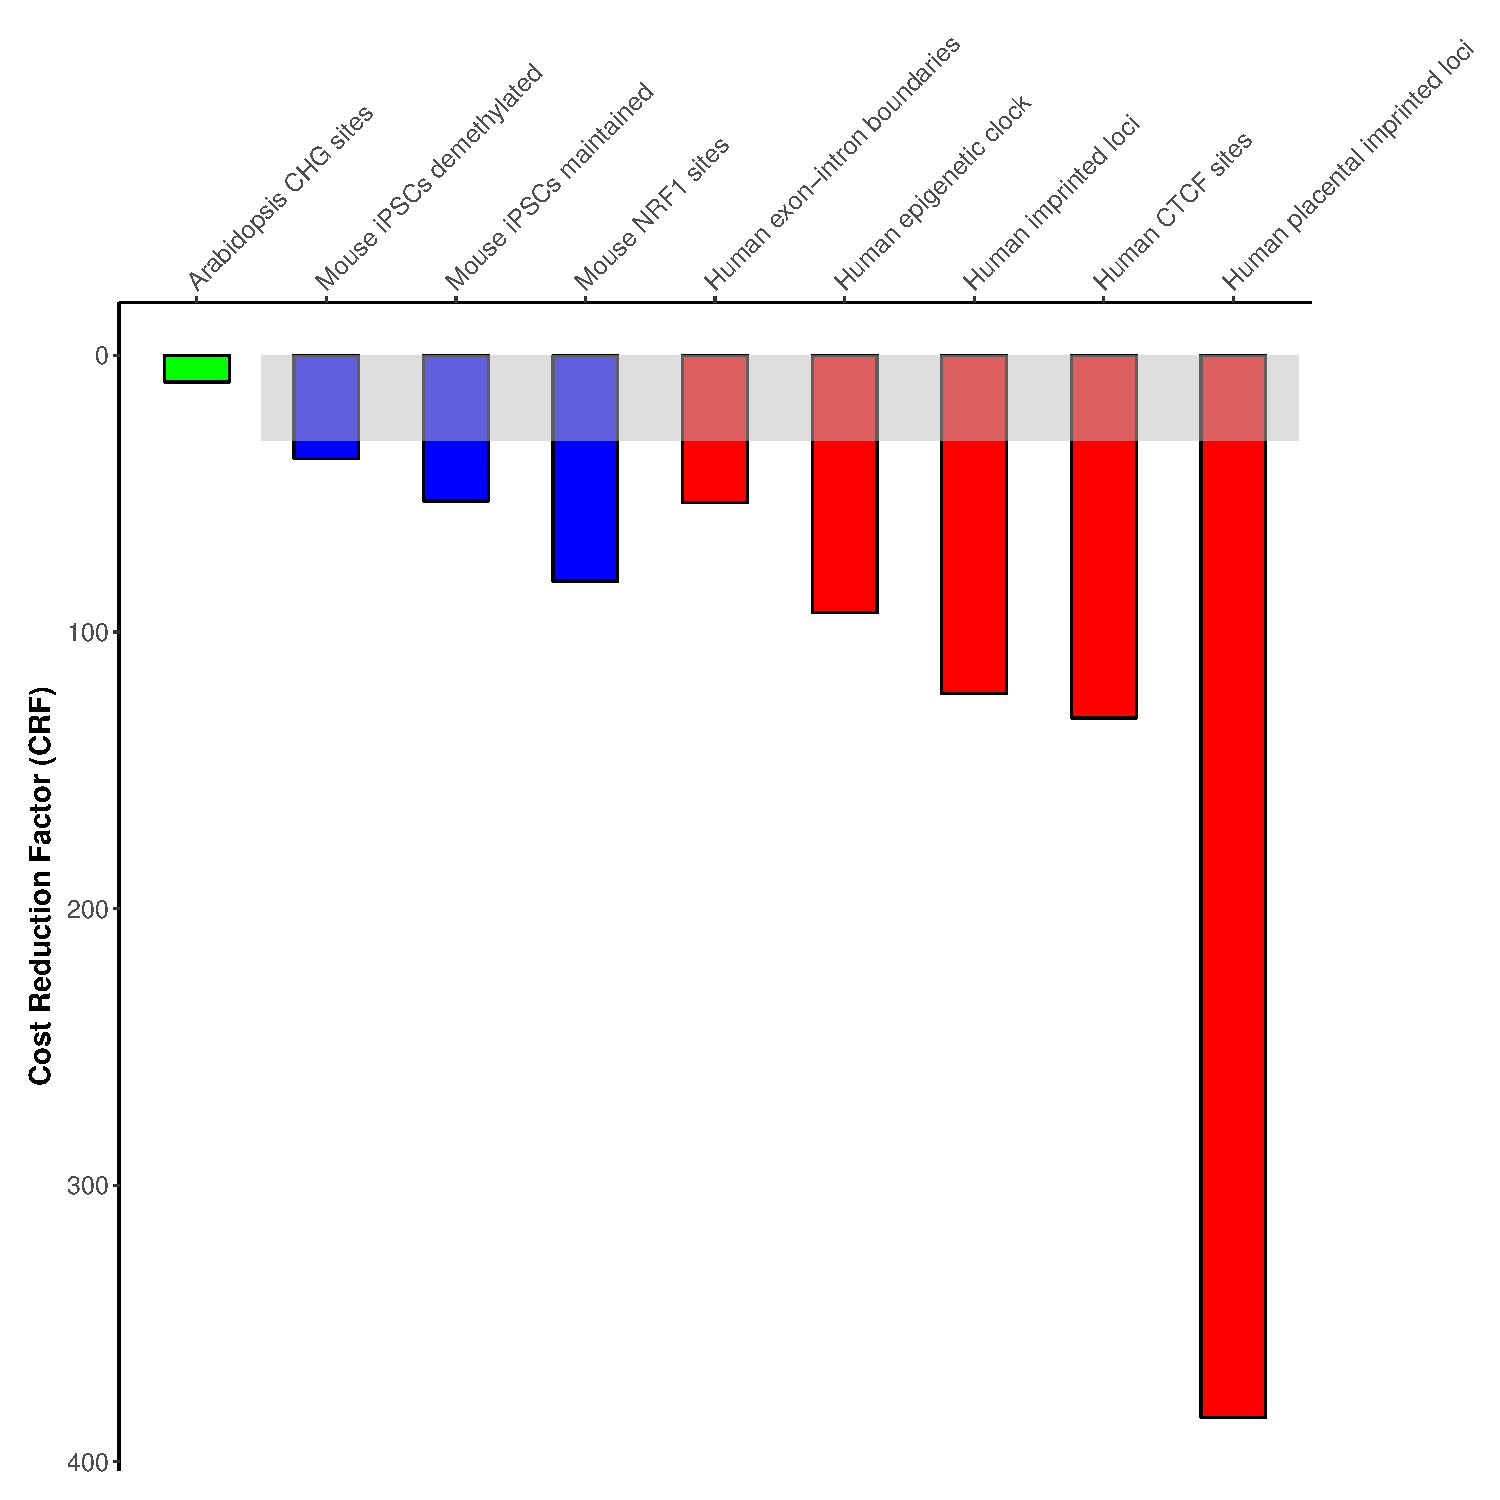
\includegraphics[width=0.5\textwidth]{C4_Fig4}
	%\vspace*{3mm}
	\caption[Running cuRRBS in different biological systems]{Running cuRRBS in different biological systems. Barplot showing the values for the \textit{Cost Reduction Factor} (\textit{CRF}) in the different biological systems that were tested (see Fig.~\ref{fig:sc4_fig5}) \cite{Horvath2013,Hanna2016,Milagre2017,Kawakatsu2016,Maurano2015,LevMaor2015,Domcke2015}. The colours in the bars represent the different species interrogated (green: \textit{Arabidopsis thaliana}, blue: \textit{Mus musculus}, red: \textit{Homo sapiens}). The \textit{CRF} for the traditional RRBS protocol (MspI in the human genome, using a bead size selection step of 20-800 bp, $CRF = 30.65$) is displayed as a grey area, which is not compared with the \textit{A. thaliana} system (since MspI is sensitive to CHG methylation).}
	\label{fig:c4_fig4}
\end{figure}


\smallskip

\section{Experimental validation of cuRRBS} \label{s:4.5}

\smallskip

To assess in an unbiased manner how well predictions from cuRRBS perform in an experimental setting, we employed two independent non-canonical RRBS datasets: one generated from a single enzyme (XmaI) and the other from a combination of two restriction enzymes (MspI and Taq$^\alpha$I) \cite{Tanas2017,Lim2016}. By evaluating the predictive power of cuRRBS in these two datasets, we were able to observe cuRRBS' performance in both single and double enzyme contexts and across different genomes.

\bigskip

To test the accuracy of cuRRBS predictions in the context of a single enzyme digestion, we utilised the non-canonical RRBS dataset generated from human DNA using the restriction enzyme XmaI \cite{Tanas2017}. This dataset was previously used to show that XmaI could enrich for CpG islands (\acrshort{CGI}s), while reducing the overall sequencing cost relative to MspI, making the protocol more cost-effective. To validate cuRRBS using this system, we therefore chose to enrich for all CpG sites that overlapped with a CGI (CGI-CpGs) in the human genome using a predetermined theoretical size range equivalent to the `reproducible library fragment lengths' reported in \cite{Tanas2017} (i.e. 90-185 bp). cuRRBS predicted with high accuracy the CpG sites that were observed in the experimental XmaI-RRBS dataset (Fig.~\ref{fig:c4_fig5}a). In particular, only a small proportion of the total number of CGI-CpGs should be theoretically sequenced (102253 out of 2164614), and this was indeed the case (Fig.~\ref{fig:c4_fig5}a). Furthermore, upon filtering out sites with low depth of coverage, which commonly represent noise in RRBS datasets, the sensitivity increased up to approximately 80\%. Importantly, the specificity remained constant at almost 100\% independent of the threshold set for depth of coverage (Fig.~\ref{fig:c4_fig5}b). Thus, cuRRBS produces a prediction that is relatively conservative, as highlighted by the low numbers of false positives (Fig.~\ref{fig:c4_fig5}a), at the expense of a small decrease in sensitivity.

\bigskip

Interestingly, the original theoretical size range that the study was aiming for (110-200 bp) was slightly different to the one achieved in the actual experiments (90-185 bp) \cite{Tanas2017}. We ran cuRRBS using the original size range target and obtained slightly worse results for the sensitivity but not the specificity of the prediction (Fig.~\ref{fig:sc4_fig6}). This demonstrates that the correct execution of the size selection step during the experimental protocol is key for obtaining the sites predicted by cuRRBS and highlights the importance of the \textit{robustness} variable as part of the cuRRBS output in order to judge the consequences of these experimental errors.

\begin{figure}[htbp!] 
	\centering    
	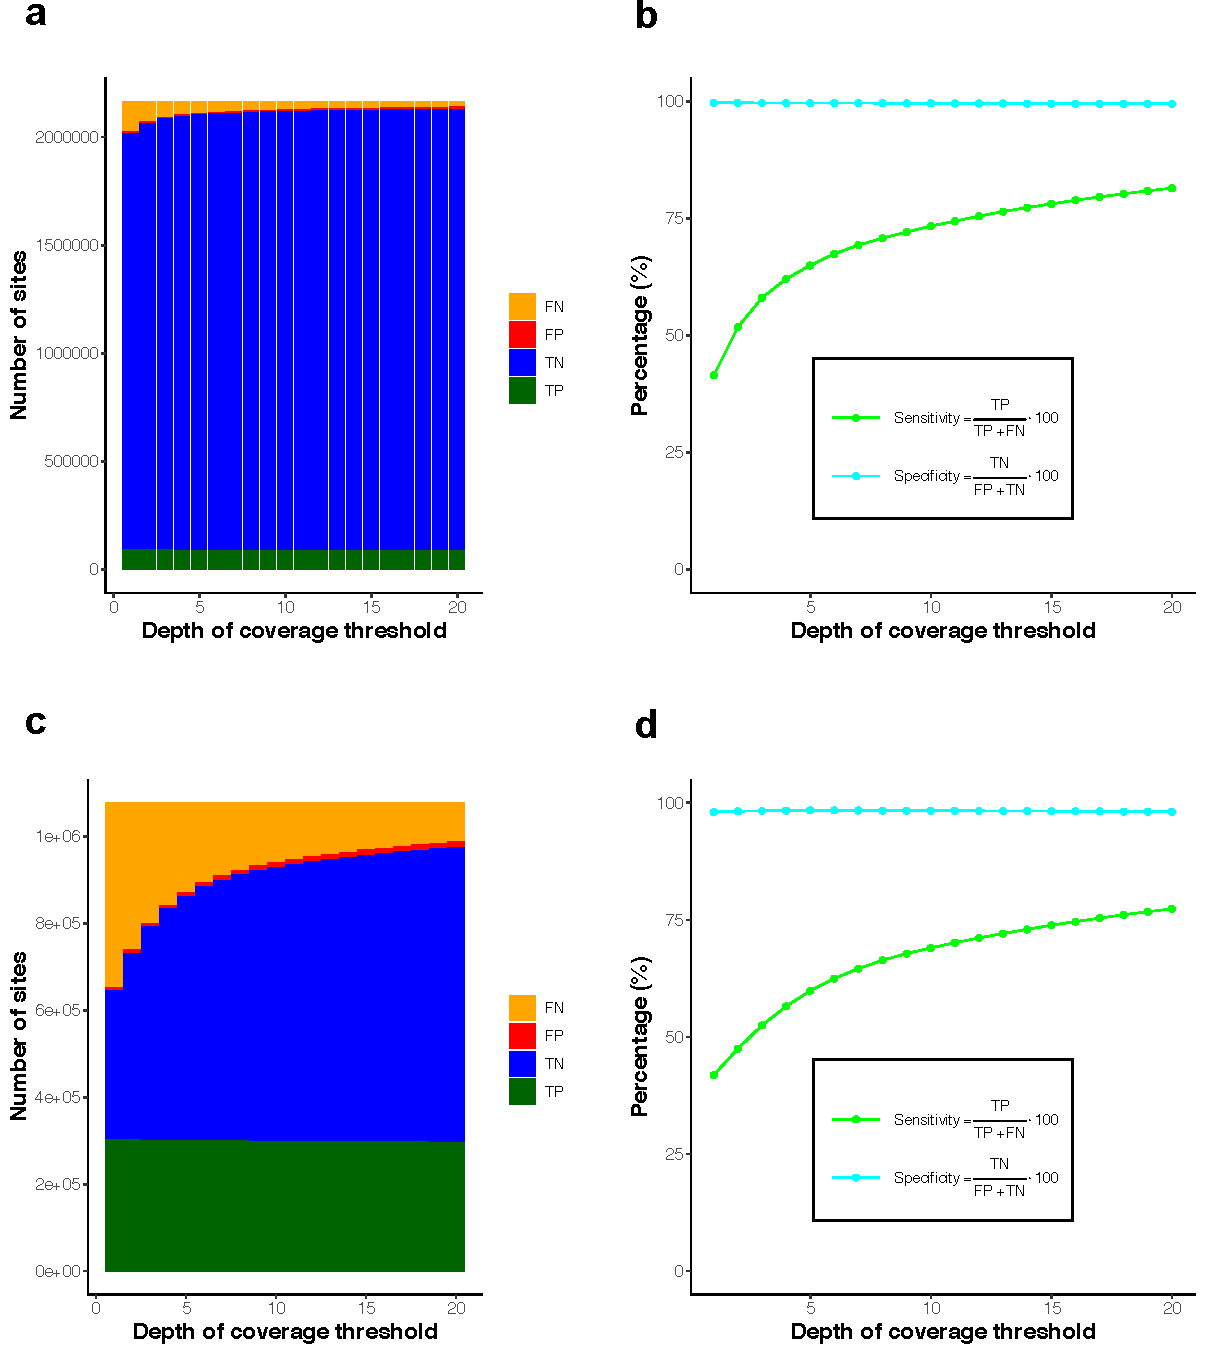
\includegraphics[width=1\textwidth]{C4_Fig5}
	\vspace*{2mm}
	\caption[Experimental validation of cuRRBS]{Experimental validation of cuRRBS. \textbf{a.} Barplots showing the number of true positives (\acrshort{TP}, in green), true negatives (\acrshort{TN}, in blue), false positives (\acrshort{FP}, in red) and false negatives (\acrshort{FN}, in orange) when comparing cuRRBS theoretical prediction with the actual XmaI-RRBS experimental data \cite{Tanas2017}. The number of sites in each category is calculated for different thresholds in the depth of coverage (number of reads covering a CpG site as reported by Bismark). cuRRBS prediction for the CpG sites in human CpG islands was obtained enforcing a theoretical size range of 90-185 bp and running the software for XmaI with all the default parameters (with a \textit{read length} of 200 bp). Legend is displayed on the right hand side. \textbf{b.} Plot showing values of cuRRBS sensitivity (in light green) and specificity (in cyan) as a function of the depth of coverage threshold employed to filter the experimental data \cite{Tanas2017}. The number of true positives (TP), true negatives (TN), false positives (FP) and false negatives (FN) are the same as in a. Legend is displayed below the plot curves. \textbf{c.} Same as in a. but for the MspI\&Taq$^\alpha$I-RRBS experimental data \cite{Lim2016}. cuRRBS prediction for the CpG sites in mouse CpG islands was obtained enforcing a theoretical size range of 80-160 bp and running the software for MspI\&Taq$^\alpha$I with all the default parameters (with a \textit{read length} of 75 bp). \textbf{d.} Same as in b. but for the MspI\&Taq$^\alpha$I-RRBS experimental data \cite{Lim2016}.}
	\label{fig:c4_fig5}
\end{figure}

\bigskip

To test the accuracy of cuRRBS predictions in the context of a double enzyme digestion, we utilised the non-canonical RRBS dataset generated from mouse DNA using the restriction enzymes MspI and Taq$^\alpha$I \cite{Lim2016}. To compare the accuracy of cuRRBS prediction in this double enzyme system to that of the XmaI-RRBS system, we again ran cuRRBS for CGI-CpGs, this time in the mouse genome with a theoretical size range of 80-160 bp \cite{Lim2016}. cuRRBS predicted with high accuracy the CpG sites that were observed in this double enzyme experiment (Fig.~\ref{fig:c4_fig5}c). In addition, the results for sensitivity and specificity were very similar to the ones reported for the XmaI-RRBS dataset (Fig.~\ref{fig:c4_fig5}d). Therefore, we conclude that cuRRBS produces robust predictions for the sites of interest that will be sequenced in RRBS protocols both for single and double enzyme combinations independent of the genome under study.

\bigskip

Lastly, the number of fragments that were theoretically recoverable in each of our experimental systems ranged from $NF = 12780$ (for XmaI) to $NF = 331058$ (for MspI and Taq$^\alpha$I). This represents approximately a 30-fold difference in the number of recoverable fragments and demonstrates that cuRRBS predictions, even for low $NF$ values, are experimentally feasible. Importantly, in the nine theoretical examples that we report (Fig.~\ref{fig:sc4_fig5}), the number of fragments required by each cuRRBS protocol ranges from 107248 to 974050. Thus, the number of fragments required to achieve the stated $CRF$ comfortably exceeds the minimum experimentally validated $NF$ value (>8-fold). 

\smallskip

\section{Conclusions and future directions}

\smallskip

cuRRBS provides a new framework that allows the user to optimise RRBS for the biological system of interest by using novel combinations of restriction enzymes. Therefore, cuRRBS makes the study of DNA methylation more affordable across all species for which genomic sequences are available. Furthermore, it can open the door to the design of future studies in a clinical context \cite{Lee2014}, which require cost-effective and robust protocols.

\bigskip

Currently, cuRRBS only considers combinations of up to two restriction enzymes. However, in the future, it would be possible to adapt the software to explore combinations that contain higher numbers of enzymes, which could theoretically allow targeting the sites of interest even more efficiently \cite{Bystrykh2013}. Moreover, there are several methods that are able to impute DNA methylation levels in sites that are not covered experimentally \cite{Zhang2015,Angermueller2017}. These methods could expand the set of sites of interest that are finally measured by making use of the additional DNA methylation information that is retrieved in a cuRRBS experiment. 

\bigskip

Finally, the potential of restriction enzymes to target different genomic coordinates is not limited to DNA methylation. As such, it would be conceivable for cuRRBS to be adapted to enrich for SNPs of interest \cite{Davey2011,Davey2011a} or to optimise chromosome conformation capture techniques \cite{Naumova2012,Dekker2013}. By reducing the cost associated with sequencing, we believe that cuRRBS will help to democratise high-throughput genomic studies. 

\smallskip

\section{Additional methods} \label{s:4.7}

\subsection*{Restriction enzymes annotation}

All the information regarding the commercially-available restriction enzymes that are used by cuRRBS was extracted from REBASE \cite{Roberts2005,Roberts2015}. Restriction enzymes were grouped in isoschizomer families (i.e. enzymes that recognise the same sequence and generate identical fragment length distributions) and each enzyme was manually annotated for different types of methylation-sensitivity (CpG, CHG, \acrshort{CHH}). Only isoschizomer families that contained at least one methylation-insensitive enzyme were considered for the examples described here.

\subsection*{Genome assemblies and genomic annotation}

All the analyses presented here were performed in the following genome assemblies: \textit{Homo sapiens} (hg38), \textit{Mus musculus} (mm10) and \textit{Arabidopsis thaliana} (TAIR10). Scaffolds not assembled into the main chromosomes were discarded. Genomic annotation for the human genome (hg38) was obtained from GENCODE (v25, basic gene annotation) \cite{Harrow2012}, with the exception of CpG islands (CGIs), which were extracted from the UCSC Genome Browser \cite{Bock2007}. GC content and CpG content were calculated, around each restriction enzyme cleavage site, taking windows of  ± 25 bp and ± 500 bp respectively. For each enzyme, the mean of all cleavage sites was calculated to obtain the mean GC content and the mean CpG content. Intragenic regions were defined as those regions within ± 2.5 \acrshort{kb} of a protein-coding gene, whilst the rest of the genome was considered to be intergenic. CpG shores were defined as regions 0 to 2 kb away from CGIs in both directions and CpG shelves as regions 2 to 4 kb away from CGIs in both directions \cite{Zhang2015}. Promoters were defined as encompassing a 3 kb region (2.5 kb upstream and 0.5 kb downstream of the  \acrshort{TSS}) relative to the TSS of all protein-coding transcripts in GENCODE, similar to the strategy used in Taher \textit{et al.} \cite{Taher2013}. Genomic annotation for the CGIs in the mouse genome (mm10) was also obtained from the UCSC Genome Browser \cite{Bock2007}. All annotations were handled using the \textit{pybedtools} library \cite{Quinlan2011,Quinlan2010}.

\subsection*{Performing \textit{in silico} digestions of a given genome}

We used the \textit{Restriction} package from Biopython v1.68 to digest the different genomes with the appropriate restriction enzymes \textit{in silico} \cite{Cock2009}. Only the first member of a given isoschizomer family (which contained at least one methylation-insensitive enzyme) was processed to avoid redundant computations. The output of the \textit{in silico} digestions was stored (pre-computed files) and subsequently read by cuRRBS when needed to reduce the computational time (see `cuRRBS heuristics and computational efficiency'). When assessing enzyme combinations, the information from the appropriate individual pre-computed files (i.e. the genomic coordinates where the enzyme theoretically cuts) were combined by the software to compute all the necessary variables.

\subsection*{cuRRBS' enzyme flexibility}

To ensure the user has full control over the enzymes that cuRRBS will use to derive the desired enrichments, one of the inputs given to cuRRBS is an enzyme annotation file. This file contains the desired isoschizomer families that the user wishes to be tested by cuRRBS. In my \href{https://github.com/demh/cuRRBS/tree/master/utils}{GitHub repository} we have already defined enzyme annotation files for enzymes that are methylation-insensitive in a CG context and in CG, CHG and CHH contexts \cite{Martin-Herranz2017}. However, it is also possible for the user to define a personalised set of enzymes by providing a self-generated annotation file. This can be useful, for instance, to reduce the chance of any star activity in the reported cuRRBS protocols.

\bigskip

In addition, the output file from cuRRBS contains, by default, 30 cuRRBS protocols that would enrich for the user's sites of interest. Therefore, the user can determine which enzyme combination and size range would be the simplest and most appropriate for the given application. This provides the user with the opportunity to consider experimental factors that may complicate the protocol, such as buffer compatibility and whether consecutive digestions would be required.

\subsection*{Flexible user-defined cuRRBS parameters}

cuRRBS contains a number of user-defined parameters to ensure the greatest possible flexibility and ease of use. A table of these parameters is provided to highlight the versatility that the user has and why such versatility is useful (Table~\ref{table:c4_table1}).

\begin{table}
	%\centering
	\small
	\begin{tabular}{ p{5cm} p{6.5cm} p{1cm} p{1.5cm} }
		\toprule
		\textbf{cuRRBS parameter (abbrev.)} & \textbf{Significance} & \textbf{Default} & \textbf{Range} \\ 
		\midrule
		Enzymes to check (-e) &  Defines the enzymes (isoschizomer families) that cuRRBS will look at & -  & -  \\
		
		Annotation for the sites of interest (-a) & Allows identification and weighting of the sites of interest & - & - \\
		
		Read length (-r) & Defines the positions in the theoretical fragments that can be `seen' after sequencing & - & 30-300 \\
		
		Adapters size (-s) & Ensures correct experimental size selection & - & - \\
		
		C\_Score constant (-c) & Sets the minimum acceptable $Score$ & - & 0-1  \\
		
		Genome size (-g) & Needed to calculate the $CRF$ & - & - \\
		
		C\_NF/1000 constant (-k) & Sets the minimum acceptable $CRF$ & 0.2 & 0-1 \\
		
		Experimental error (-d) & Sets the assumed experimental error ($\delta$) & 20 & 5-500  \\
		
		Size range breadth (-b) & Constrains the breadth of the size range & 980 & - \\
		
		Output size (-t) & Defines the number of cuRRBS protocols the user can compare & 30 & - \\
		
		Site IDs (-i) & Enables the identification of the recovered sites of interest & No & - \\
		\bottomrule
	\end{tabular}
	\vspace*{3mm}
	\caption[Flexible user-defined cuRRBS parameters]{Flexible user-defined cuRRBS parameters. This table details the flexible user-defined parameters that cuRRBS will accept as arguments. The cuRRBS parameter full name and command line abbreviation (in brackets) are provided alongside a simplified description of the significance of these arguments to the user. Where applicable, the defaults and ranges of these arguments are also detailed.}
	\label{table:c4_table1}
\end{table}


\subsection*{cuRRBS heuristics and computational efficiency}

cuRRBS employs several strategies to reduce the computational time needed in each run:

\begin{itemize}
	
	\item Restriction enzymes are grouped in isoschizomer families. Since isoschizomers generate the same genomic digestions, only one member of each family needs to be processed. 
	
	\item \textit{In silico} digestions are read from pre-computed files. Digesting the genomes would be a limiting factor in the cuRRBS pipeline. The user can download the pre-computed files \cite{Martin-Herranz2017} and the information that they contain is read every time that an enzyme needs to be assessed.
	
	\item The number of size ranges that are sampled is minimised. Since the experimental size selection step is generally imperfect, size ranges are sampled with a sliding window whose `resolution' is equivalent to the experimental error specified by the user. 
	
	\item Parallelization. cuRRBS can use several cores to decrease the \acrshort{CPU} time.

\end{itemize}

Moreover, we have observed that, in many enzyme combinations, one of the enzymes is providing most of the enrichment for the sites of interest, while the second one complements the targeting. Therefore, it would be possible to implement a `heuristic' mode, where only those enzymes that perform well individually are used as `seeds' to construct combinations (as opposed to the current implementation, where all the enzyme combinations are checked exhaustively). This could further reduce the computational time, especially if combinations of more than two enzymes were being evaluated. 

\bigskip

The CPU time required by cuRRBS depends on several parameters, including the number of enzymes checked, the experimental error, the number of sites of interest or the genome size (Fig.~\ref{fig:sc4_fig7}). The RAM used will be approximately equal to the size of the pre-computed files that are read by the software. A standard cuRRBS run (e.g. for a few thousand sites of interest in the human genome, checking 128 CpG methylation-insensitive isoschizomer families) takes around 0.5-1 hours and uses around 4 \acrshort{GB} \acrshort{RAM}, which allows the user to easily run it on a dual-core laptop or desktop computer. 


\subsection*{Obtaining the sites of interest for different biological systems}

We have tested \textit{in silico} the ability of cuRRBS to enrich for the sites of interest in a selection of different biological systems where DNA methylation has an important functional role. In some of these systems, described below, previous analysis was performed in order to obtain the genomic coordinates for the sites:

\begin{itemize}

	\item Exon-intron boundaries in human. Exons and introns were obtained from protein-coding genes using GENCODE annotation data. Those CpG sites that were found within ± 5 bp of a canonical splice site (5'-GT, 3'-AG) were selected.
	
	\item Epigenetic clock in human. These sites were obtained from the Horvath epigenetic clock \cite{Horvath2013} and were lifted over to hg38 \cite{Kuhn2012} before running cuRRBS.
	
	\item Canonical and placental imprints in human. These loci were obtained from Hanna \textit{et al.} \cite{Hanna2016}. The sites were lifted over to hg38 \cite{Kuhn2012} and the CpG sites were then extracted for the analysis. 
	
	\item \acrshort{CTCF} binding sites in human. We obtained the CpG sites that overlap with \textit{in vivo} CTCF binding sites. Peaks from sites that seem to be affected by methylation (upregulated, reactivated) were kindly provided by Dr. M. T. Maurano \cite{Maurano2015}. We scanned the peaks for high-scoring motifs according to the CTCF JASPAR model \cite{Zhang2015a}. Finally, we extracted those CpGs that were found in positions 5 and 15 of the motif, whose methylation status is supposed to influence the binding of the transcription factor \cite{Maurano2015}. 
	
	\item Induced pluripotent stem cells (\acrshort{iPSCs}) demethylated and maintained sites in mouse. These were obtained by comparing mouse embryonic fibroblasts (\acrshort{MEFs}) to iPSCs as described previously \cite{Milagre2017}, with an additional filter for magnitude of methylation change (>50$\%$ methylation change).
	
	\item \acrshort{NRF1} binding sites in mouse. We obtained the CpG sites that overlap with \textit{in vivo} NRF1 binding sites in mouse. \acrshort{ChIP-seq} data was processed as described in the original publication \cite{Domcke2015}, where peaks were called using Peakzilla \cite{Bardet2013}. We took as our final set of peaks the overlap between the two \acrshort{TKO} replicates. Next, we scanned the peaks for high-scoring motifs according to the NRF1 JASPAR model \cite{Zhang2015a}. Finally, we extracted those CpGs that were found in positions 2 and 8 of the motif, whose methylation status is supposed to influence the binding of the transcription factor \cite{Zhang2015a}.
	
	\item CHG sites in \textit{Arabidopsis thaliana}. Non-CpG DMRs arising from the epigenomic diversity between \textit{Arabidopsis thaliana} accessions were obtained from Kawakatsu \textit{et al.} \cite{Kawakatsu2016}. The coordinates for C sites in non-CpG context were extracted.
	
	
\end{itemize}

In all the cases the sites were equally weighted ($w_i = 1$), with the exception of the human epigenetic clock system, where the sites were assigned the absolute value of the weights in the linear model \cite{Horvath2013}. All the site annotation files can be found in my \href{https://github.com/demh/cuRRBS/tree/master/examples}{GitHub repository} \cite{Martin-Herranz2017}


\subsection*{Running cuRRBS for the different biological systems}

cuRRBS was run in the different systems described above using the default parameters ($k = 0.2$, $d = 20$, $b = 980$, $t = 30$), for a \textit{read length} (\textit{r}) of 75 bp and a \textit{Score threshold} (\textit{c}) of 0.25. In the mouse and human examples we considered 128 isoschizomer families that contained enzymes that were not sensitive to CpG methylation. In the case of \textit{Arabidopsis thaliana} we used 28 isoschizomer families that contained enzymes that were not sensitive to 5mC in any context (\acrshort{CG}, CHG, CHH).


\subsection*{Mapping of RRBS samples}

XmaI-RRBS data generated on the Ion Torrent platform \cite{Tanas2017} and MspI\&Taq$^\alpha$I -RRBS data generated on the Illumina HiSeq platform \cite{Lim2016} were quality trimmed using Trim Galore (www.bioinformatics.babraham.ac.uk/projects/trim\_galore/) and had base pairs removed from the 3' end to avoid including filled-in nucleotides with artificial methylation states (the filled-in XmaI, MspI and Taq$^\alpha$I cut sites include the nucleotide sequence CCGG, CG and CG respectively). The data was then mapped to the human genome (for XmaI data, parameters: --non\_directional) or the mouse genome (for MspI\&Taq$^\alpha$I  data, parameters: --directional) using Bismark (0.18.0) \cite{Krueger2011}. In each of the two cases data from different experiments or replicates was merged into the same FASTQ file prior to quality trimming.

\subsection*{Estimating cuRRBS' sensitivity and specificity }

We assessed the performance of cuRRBS predictions in two independent experimental datasets \cite{Tanas2017,Lim2016} (see section~\ref{s:4.5}). We ran cuRRBS fixing the theoretical size ranges tested to the ones reported in the publications \cite{Tanas2017,Lim2016} and we used as our sites of interest the CpGs that overlapped with CpG islands (CGI-CpGs) in the human \cite{Tanas2017} and the mouse genomes \cite{Lim2016} respectively. From the cuRRBS output files we recovered the IDs of the sites that should be theoretically sequenced. Moreover, using the experimental RRBS data \cite{Tanas2017,Lim2016}, we could obtain the IDs of the sites that were actually sequenced (filtered by a given depth of coverage threshold). Afterwards, we calculated the following variables for each one of the datasets:

\begin{itemize}
	
	\item True positives (TP): number of CGI-CpGs that cuRRBS predicted to be sequenced and were indeed found in the RRBS data.
	
	\item True negatives (TN): number of CGI-CpGs that cuRRBS predicted to be absent and were not found in the RRBS data.
	
	\item False positives (FP): number of CGI-CpGs that cuRRBS predicted to be sequenced but were not found in the RRBS data.
	
	\item False negatives (FN): number of CGI-CpGs that cuRRBS predicted to be absent but were found in the RRBS data.
	
\end{itemize}

Finally, we estimated the sensitivity and specificity, for a given dataset, as follows:

\begin{align}
Sensitivity = \frac{TP}{TP+FN} \cdot 100
\end{align}

\begin{align}
Specificity = \frac{TN}{FP+TN} \cdot 100
\end{align}

\subsection*{Software availability}

cuRRBS and its documentation are freely distributed under GNU General Public License v3.0 and can be accessed in my \href{https://github.com/demh/cuRRBS/}{GitHub repository} \cite{Martin-Herranz2017}.